\documentclass{ecnreport}

\stud{Master 1 CORO / Option Robotique}
\topic{Robot Operating System (2)}
\author{O. Kermorgant}

\begin{document}

\inserttitle{Robot Operating System\newline (for lab assistants)}

\insertsubtitle{How to setup Baxter}

\section{General commands on Baxter and ROS 1/2}

The computers use the \okt{ros\_management\_tools} to handle the ROS version and connection on another ROSMASTER (ROS 1).

Here are the main commands:
\begin{bashcodelarge}
ros1ws  # use ROS 1
ros2ws # use ROS 2
ros_baxter # ROS 1 uses Baxter's ROSMASTER
ros_turtle 1  # ROS 2 will connect to turtlebot1's ROS_DOMAIN_ID
ros_reset # ROS 1 uses local ROSMASTER, ROS 2 uses local domain ID only
\end{bashcodelarge}

All these commands only have to be typed once. They will be forwarded to any new terminal, and to QtCreator is it is open with the corresponding icon ("for ROS 1" / "for ROS 2").

\section{Use in simulation}

In the simulation, only ROS 2 is needed. Hence the first step is:
\begin{bashcodelarge}
ros2ws && ros_reset
\end{bashcodelarge}

The simulation can be run with:
\begin{bashcodelarge}
 ros2 launch baxter_simple_sim sim_launch.py
\end{bashcodelarge}

\section{Use on the real robot}

The real robot first needs to be run once. Then, each student must run their own bridge between ROS 1 and ROS 2.

\subsection{Running the robot}

Baxter is a pure ROS 1 robot so running it is done on ROS 1:
\begin{bashcodelarge}
 # power on!
 ros1ws && ros_baxter # use ROS 1 on Baxter's ROSMASTER
 rosrun baxter_tools enable_robot.py -e  # enable
 rosrun baxter_tools tuck_arms.py -u # untuck the arms
\end{bashcodelarge}

\subsection{Allowing (or not) several publishers on the same topic}

On the ROS 1 side, if several people publish on the joint command topics they will all move the robot.

\begin{center}
 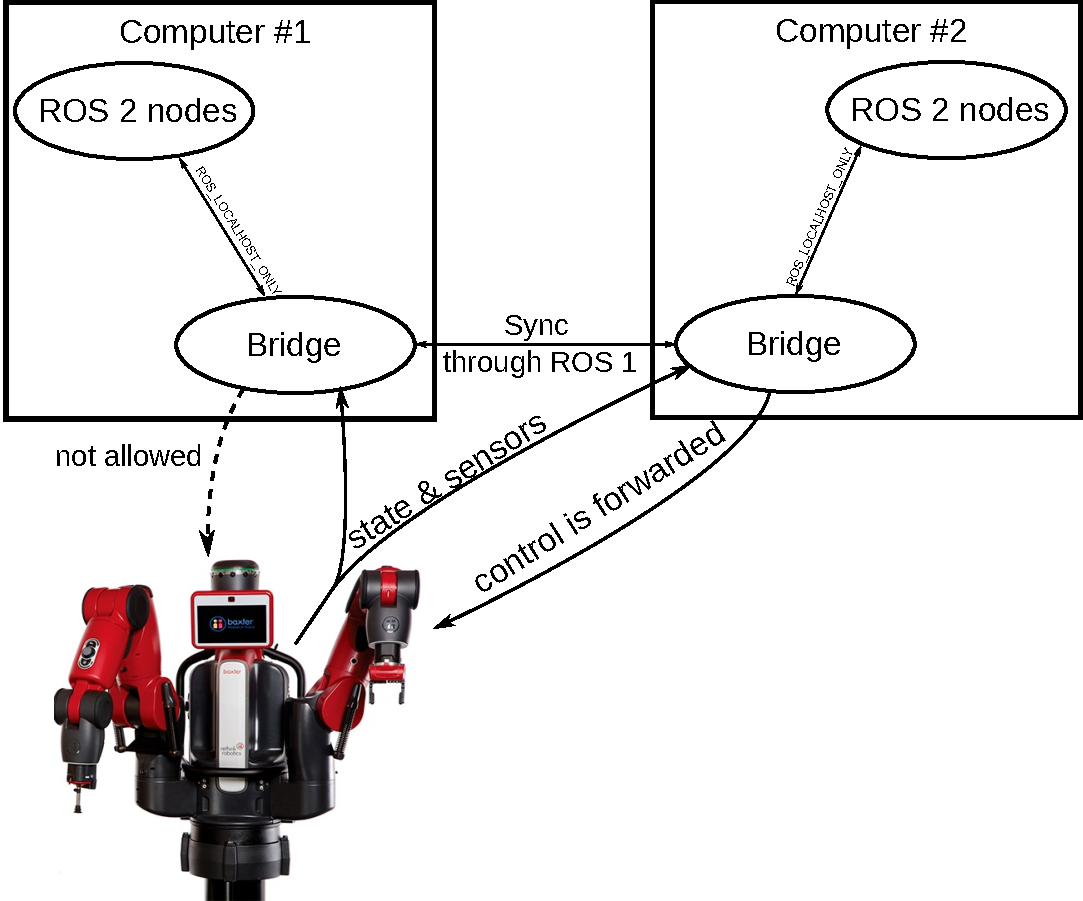
\includegraphics[width=.5\linewidth]{sync}
\end{center}


This can be controlled on the ROS 2 side as \okt{baxter\_bridge} checks for a special parameter. In practice, {\bf only the first lab} should allow all students to control the arm at the same time. To ensure this, type:
 \begin{bashcodelarge}
 ros1ws && ros_baxter # so that your ROSMASTER is Baxter
 rosparam set allow_multiple true
\end{bashcodelarge}

\subsection{Running the bridge}

Baxter bridge in a ROS 2 and ROS 1 node, but should be run through ROS 2. The ROS 1 part still needs to connect on Baxter's ROSMASTER:
 \begin{bashcodelarge}
 ros2ws && ros_baxter # use ROS 2 but set ROS 1 ROSMASTER to Baxter
 ros2 launch baxter_bridge baxter_bridge_launch.py
\end{bashcodelarge}

Each student should have their own bridge, that will communicate locally on ROS 2 but with Baxter on ROS 1.

\subsection{Powering off}

\begin{bashcodelarge}
 ros1ws && ros_baxter # use ROS 1 on Baxter's ROSMASTER
 rosrun baxter_tools tuck_arms.py -t # tuck the arms
 rosrun baxter_tools enable_robot.py -d  # disable
 # power off by holding the power button for 2-3 s
\end{bashcodelarge}


\end{document}
